\documentclass[aspectratio=169,10pt]{beamer}
\usetheme{metropolis}
\metroset{sectionpage=none}
\usepackage{tikz}
\usetikzlibrary{arrows.meta,positioning,shapes.geometric,fit,calc}
\usepackage{listings}
\lstset{basicstyle=\ttfamily\scriptsize,breaklines=true,columns=fullflexible,keepspaces=true,frame=single,framerule=0.2pt}
\newcommand{\nn}{\textsc{nixnan}}
\tikzset{box/.style={draw,rounded corners,align=center,inner sep=4pt,font=\scriptsize,fill=blue!6},
 gbox/.style={box,fill=green!10},rbox/.style={box,fill=red!8},arr/.style={-{Stealth},thick},
 lbl/.style={font=\tiny,align=center}}
\title{How \nn{} works: from load to the first HMMA report}
\subtitle{SC26 tutorial walk-through, using the reaction--diffusion demos}
\author{Ganesh Gopalakrishnan}
\date{2026-10-19}
\begin{document}
\maketitle

\begin{frame}{Roadmap}
\begin{enumerate}\small
\item Setup, and the one environment trap
\item Callback architecture (NVBit $\leftrightarrow$ \nn)
\item Lifecycle of the tool
\item First kernel launch: how instrumentation happens
\item Compact encoding: \texttt{instructions.json} $\to$ \texttt{reginfo} word
\item The two injected calls (\texttt{IPOINT\_AFTER}/\texttt{BEFORE})
\item Device side: classify, OR, count, push
\item GPU$\to$CPU channel, doorbell, receiver thread, sentinel
\item End-of-run report
\item \textbf{Part A:} an ordinary SASS instruction (\texttt{HFMA2} in \texttt{rd\_nixnan})
\item \textbf{Part B:} \texttt{HMMA.16816.F16} in \texttt{rd\_tc}
\end{enumerate}
\end{frame}

\begin{frame}[fragile]{Setup, and the trap}
\begin{lstlisting}
env -u LD_LIBRARY_PATH \
  LINE_INFO=1 PRINT_ILL_INSTR=1 TOOL_VERBOSE=1 \
  LOGFILE=latex/data/partA-scalar.log \
  LD_PRELOAD=~/repos/nixnan/nixnan.so ./rd_nixnan
\end{lstlisting}
\begin{itemize}\small
\item \texttt{LD\_PRELOAD} loads \nn{} (built on NVBit 1.8) before the CUDA runtime.
\item On this machine, with my usual \texttt{LD\_LIBRARY\_PATH} (a missing \texttt{cuda-13.2/lib64} plus a dyninst lib dir) \nn{} printed its banner and \emph{nothing else}. With \texttt{env -u LD\_LIBRARY\_PATH} the same binary reports. (Observed this session; I did not isolate which entry is at fault.)
\item An earlier driver-mismatch (kernel module 595.84 vs.\ library 595.99.02) was cured by a reboot.
\item Branch \texttt{print\_histo\_instrn}, commit \texttt{ce35185}.
\end{itemize}
\end{frame}

\section{Architecture}
\begin{frame}{Callback architecture}
\centering
\resizebox{0.97\textwidth}{!}{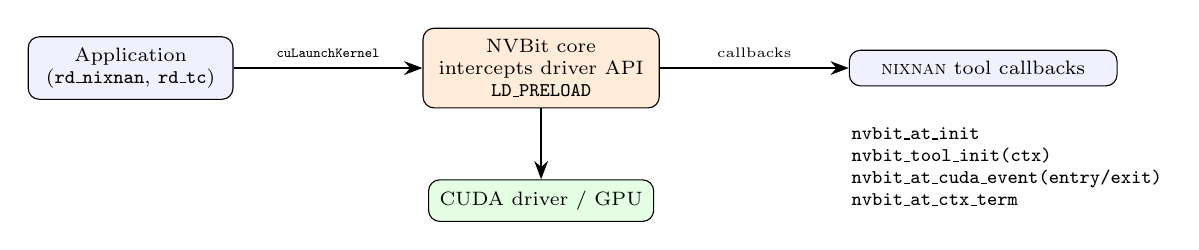
\begin{tikzpicture}[node distance=9mm and 24mm]
\node[box,minimum width=2.6cm] (app) {Application\\(\texttt{rd\_nixnan}, \texttt{rd\_tc})};
\node[box,right=of app,minimum width=3cm,fill=orange!15] (nv) {NVBit core\\intercepts driver API\\\texttt{LD\_PRELOAD}};
\node[box,right=of nv,minimum width=3.4cm] (tool) {\nn{} tool callbacks};
\node[gbox,below=of nv] (drv) {CUDA driver / GPU};
\draw[arr] (app) -- node[lbl,above]{\texttt{cuLaunchKernel}} (nv);
\draw[arr] (nv) -- node[lbl,above]{callbacks} (tool);
\draw[arr] (nv) -- (drv);
\node[font=\scriptsize,align=left,below=4mm of tool,xshift=3mm] (cbs) {%
\texttt{nvbit\_at\_init}\\
\texttt{nvbit\_tool\_init(ctx)}\\
\texttt{nvbit\_at\_cuda\_event(entry/exit)}\\
\texttt{nvbit\_at\_ctx\_term}};
\end{tikzpicture}}
\end{frame}

\begin{frame}{Lifecycle of the tool (\texttt{nixnan.cu})}
\small
\begin{description}
\item[\texttt{nvbit\_at\_init}] reads env vars via \texttt{GET\_VAR\_*} (\texttt{INSTR\_BEGIN/END}, \texttt{TOOL\_VERBOSE}, \texttt{PRINT\_ILL\_INSTR}, \texttt{SAMPLING}, \texttt{LINE\_INFO}, \texttt{LOGFILE}, \texttt{MAX\_ERRORS}, white/blacklist\dots); sets \texttt{CUDA\_MANAGED\_FORCE\_DEVICE\_ALLOC=1}; prints the banner.
\item[\texttt{nvbit\_tool\_init}] ``Initializing GPU context\dots'': builds \texttt{recorder(TABLE\_SIZE)}, \texttt{TABLE\_SIZE = $2^{17}$} entries; \texttt{channel\_host.init(0, sizeof(exception\_info), \&channel\_dev, NULL)}; starts \texttt{recv\_thread}.
\item[\texttt{nvbit\_at\_cuda\_event}, entry] for the launch APIs: \texttt{recv\_thread\_receiving = true}; \texttt{instrument\_function}; prints ``running kernel [\dots]'' the first time; \texttt{nvbit\_enable\_instrumented(\dots, sampling>0 ? count\%sampling==0 : true)}.
\item[\texttt{nvbit\_at\_cuda\_event}, exit] \texttt{cudaDeviceSynchronize()}, check \texttt{cudaGetLastError()}.
\item[\texttt{nvbit\_at\_ctx\_term}] stop and \texttt{join} the receiver, \texttt{recorder->end()}, print the report.
\end{description}
\end{frame}

\begin{frame}{First launch of a kernel: what happens}
\centering
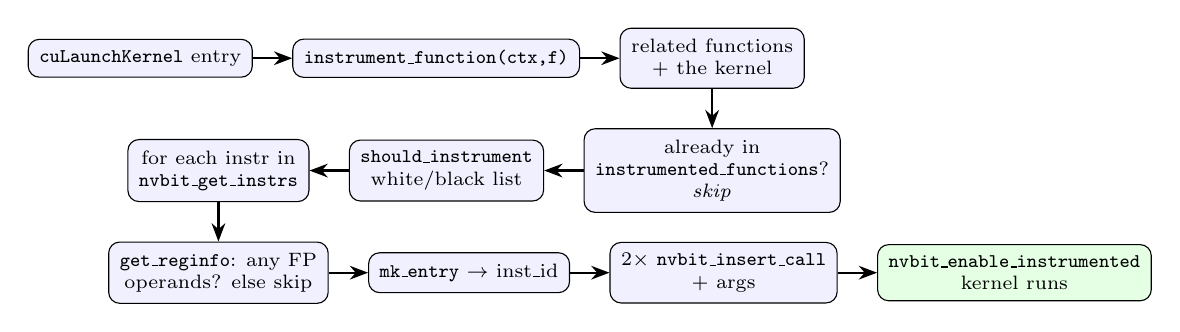
\begin{tikzpicture}[node distance=5mm,every node/.style={font=\scriptsize}]
\node[box] (a) {\texttt{cuLaunchKernel} entry};
\node[box,right=of a] (b) {\texttt{instrument\_function(ctx,f)}};
\node[box,right=of b] (c) {related functions\\+ the kernel};
\node[box,below=of c] (d) {already in\\\texttt{instrumented\_functions}?\\\textit{skip}};
\node[box,left=of d] (e) {\texttt{should\_instrument}\\white/black list};
\node[box,left=of e] (f) {for each instr in\\\texttt{nvbit\_get\_instrs}};
\node[box,below=of f] (g) {\texttt{get\_reginfo}: any FP\\operands? else skip};
\node[box,right=of g] (h) {\texttt{mk\_entry} $\to$ inst\_id};
\node[box,right=of h] (i) {2$\times$ \texttt{nvbit\_insert\_call}\\+ args};
\node[gbox,right=of i] (j) {\texttt{nvbit\_enable\_instrumented}\\kernel runs};
\draw[arr](a)--(b);\draw[arr](b)--(c);\draw[arr](c)--(d);\draw[arr](d)--(e);\draw[arr](e)--(f);
\draw[arr](f)--(g);\draw[arr](g)--(h);\draw[arr](h)--(i);\draw[arr](i)--(j);
\end{tikzpicture}

\vspace{2mm}\small Instrumentation happens once per function; later launches only toggle \texttt{nvbit\_enable\_instrumented} (SAMPLING).
\end{frame}

\section{Encoding}
\begin{frame}[fragile]{Table-driven: \texttt{instructions.json}}
\small The opcode string is matched against keys (each tried as a regex with \texttt{regex\_match}); the entry lists operand groups in SASS operand order.
\begin{lstlisting}
"HMMA.16816.F16": {"registers": [
   {"type":"f16","count":4},   // operand 0  D (destination)
   {"type":"f16","count":8},   // operand 1  A
   {"type":"f16","count":4},   // operand 2  B
   {"type":"f16","count":4} ]} // operand 3  C
"(FFMA(?:\\.FTZ)?(?:\\.(RP|RM|RZ))?(?:\\.SAT)?)": ...   // regex key
\end{lstlisting}
\begin{itemize}\small
\item \texttt{count} = number of \emph{values}; registers needed: \texttt{get\_num\_regs}: f16/bf16 $\lceil n/2\rceil$, f32 $n$, f64 $2n$.
\item Optional \texttt{"div0"} flag asks to flag zeros too.
\item The JSON is embedded in the binary as a byte array (\texttt{instructions.h}) and parsed once (nlohmann).
\item Opcodes with no entry (e.g.\ \texttt{F2FP.PACK}: grep count 0 in the JSON) are \emph{not instrumented}.
\end{itemize}
\end{frame}

\begin{frame}{One 32-bit word per operand: \texttt{reginfo}}
\centering
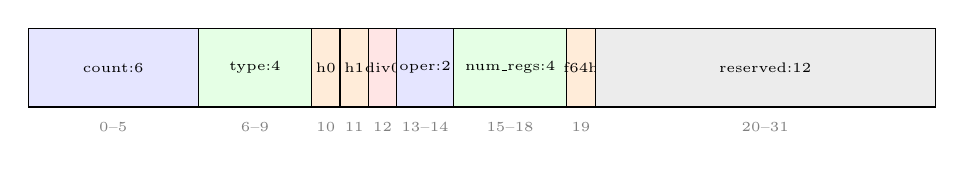
\begin{tikzpicture}[x=0.36cm,y=1cm]
\foreach \a/\b/\t/\c in {0/5/count:6/blue!10,6/9/type:4/green!10,10/10/h0/orange!15,11/11/h1/orange!15,12/12/div0/red!10,13/14/oper:2/blue!10,15/18/num\_regs:4/green!10,19/19/f64h/orange!15,20/31/reserved:12/gray!15}{
 \draw[fill=\c] (\a,0) rectangle (\b+1,1); \node[font=\tiny] at ({(\a+\b+1)/2},0.5) {\t};
 \node[font=\tiny,gray] at ({(\a+\b+1)/2},-0.25) {\a\ifnum\a=\b\else--\b\fi};}
\end{tikzpicture}

\small\raggedright Bit positions assume GCC's LSB-first bit-field allocation (my reading; not dumped from a binary).
\begin{itemize}\small
\item \texttt{static\_assert(sizeof(reginfo)==4)} so it travels as \emph{one} 32-bit call argument (\texttt{nvbit\_add\_call\_arg\_const\_val32}).
\item \texttt{type}: FP16=0, BF16=1, FP32=2, FP64=3. \texttt{operand} is 2 bits: at most 4 operands (\texttt{OPERANDS=4}).
\item \texttt{count} and \texttt{num\_regs} are signed \texttt{int} bit-fields (6 and 4 bits), so \texttt{num\_regs} is meaningful only up to 7 though \texttt{get\_reginfo} asserts $<16$.
\item \texttt{half\_h0/h1}: which half of a packed pair to inspect.
\end{itemize}
\end{frame}

\begin{frame}{Turning an operand into register reads: \texttt{get\_regs}}
\small
\begin{tabular}{@{}l>{\raggedright\arraybackslash}p{0.62\textwidth}@{}}
\textbf{Operand kind} & \textbf{What \nn{} does}\\\hline
\texttt{REG} / \texttt{UREG} & one lambda per register: \texttt{nvbit\_add\_call\_arg\_reg\_val / ureg\_val(instr, clamp(reg+i))}\\
\texttt{CBANK} & lambda: \texttt{nvbit\_add\_call\_arg\_cbank\_val(instr, id, imm\_offset+4i)}\\
\texttt{IMM\_DOUBLE} & checked on the host; prints a warning if NaN/Inf/subnormal; no runtime arg\\
\texttt{IMM\_UINT64} & ignored (\texttt{num\_regs=0})\\
\texttt{GENERIC} & text-matched for NAN/INF, warning only\\
\end{tabular}

\medskip
The lambdas are \emph{deferred}: they are stored in the \texttt{reginsertion} vectors and executed only \emph{after} the call's fixed arguments have been added, so argument order is correct. \texttt{f64high} opcodes (suffix \texttt{64H}) start one register lower.
\end{frame}

\begin{frame}{Book-keeping on the host: \texttt{recorder::mk\_entry}}
\small
Each instrumented instruction gets a dense \texttt{inst\_id} (the table index) and a \texttt{host\_entry}:
\begin{itemize}
\item SASS string (\texttt{instr->getSass()}), function name (\texttt{cut\_kernel\_name}), up to 4 operand types.
\item Source location, if \texttt{LINE\_INFO}: \texttt{nvbit\_get\_line\_info(ctx,f,offset,\dots)} under a temporary \texttt{SIGSEGV} handler (prints ``try LINE\_INFO=0'' and exits if NVBit crashes reading debug info).
\end{itemize}
Device counters: \texttt{device\_errors} = \texttt{cudaMalloc}'d array of $2^{17}\!\cdot\!2^{7}$ \texttt{uint32} zero-initialised; index
\[ \texttt{id}\,\ll 7 \;|\; \texttt{op}\,\ll 5 \;|\; \texttt{exce}\quad(\text{SH\_AMT}=\text{EXCEBITS}+\text{OPBITS}=5+2). \]
The ID is the only thing the GPU needs to send back; strings never leave the host.
\end{frame}

\section{Injection}
\begin{frame}[fragile]{Two injected calls per instruction}
\begin{columns}\begin{column}{0.5\textwidth}\small
\textbf{\texttt{IPOINT\_AFTER}}: operand \textbf{0} (the destination)
\begin{lstlisting}
nvbit_insert_call(instr,"nixnan_check_regs",
                  IPOINT_AFTER);
guard_pred_val
const64 recorder->device_recorder
const32 inst_id
const64 &channel_dev
const32 1 + rfuns.size()   // arg_count
const32 reginfo(op 0)
reg values via lambdas...
\end{lstlisting}
\end{column}\begin{column}{0.5\textwidth}\small
\textbf{\texttt{IPOINT\_BEFORE}}: operands \textbf{1\dots n} (sources)
\begin{lstlisting}
nvbit_insert_call(instr,"nixnan_check_regs",
                  IPOINT_BEFORE);
guard_pred_val
const64 device_recorder
const32 inst_id
const64 &channel_dev
const32 sum(num_regs) + (#ops-1)
{const32 reginfo(op i); regs...}*
\end{lstlisting}
\end{column}\end{columns}
\smallskip\small Destination is read \emph{after} the instruction (the result), sources \emph{before} (so overwritten registers, e.g.\ \texttt{R26} as both C and D, are seen with their old value).
\texttt{nvbit\_add\_call\_arg\_guard\_pred\_val} passes the guard predicate: predicated-off threads do nothing.
\end{frame}

\section{Device}
\begin{frame}[fragile]{\texttt{nixnan\_check\_regs} on the GPU (\texttt{inject\_funs.cu})}
\small
\begin{enumerate}
\item \texttt{if (!pred) return;}  \quad active mask by \texttt{\_\_ballot\_sync}; \texttt{first\_laneid = \_\_ffs(mask)-1}.
\item \texttt{va\_arg} loop: read a \texttt{reginfo}, then \texttt{count} values; classify by \texttt{type}:
\end{enumerate}
\begin{tabular}{@{}ll@{}}
FP16 & \texttt{half2\_classify(val,h0,h1,div0)}; consumes 2 values per register\\
BF16 & \texttt{bf162\_classify(\dots)}\\
FP32 & \texttt{float\_classify(val,div0)}\\
FP64 & two words (low, high) $\to$ \texttt{double\_classify}\\
\end{tabular}
\begin{enumerate}\setcounter{enumi}{2}
\item Result bits OR-ed into \texttt{exces[operand]}: \texttt{E\_NAN=1, E\_INF=2, E\_NINF=4, E\_SUB=8, E\_DIV0=16}.
\item Shuffle-OR across the 32 lanes (\texttt{\_\_shfl\_sync} loop) so every lane has the warp's verdict.
\item First active lane: for each operand with \texttt{exce!=0}: \texttt{old = recorder.record(id,exce,op)} = \texttt{atomicAdd(device\_errors+idx,1)}.
\item \textbf{Only if \texttt{old==0}} (first time this (instr, operand, flag-set) is seen) push \texttt{exception\_info} to the channel (twice, see later).
\end{enumerate}
Repeats are therefore only \emph{counted}, never transmitted: that is the ``(N repeats)'' in the final report.
\end{frame}

\begin{frame}{The packet: \texttt{exception\_info}}
\centering
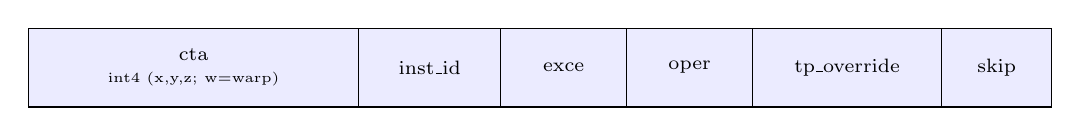
\begin{tikzpicture}[y=1cm]
\foreach \a/\b/\t in {0/4.2/cta\\{\tiny int4 (x,y,z; w=warp)},4.2/6/inst\_id,6/7.6/exce,7.6/9.2/oper,9.2/11.6/tp\_override,11.6/13/skip}{
\draw[fill=blue!8] (\a,0) rectangle (\b,1); \node[font=\scriptsize,align=center] at ({(\a+\b)/2},0.5){\t};}
\end{tikzpicture}

\small\raggedright
\begin{itemize}
\item Fixed-size struct; \texttt{CHANNEL\_SIZE = sizeof(exception\_info)}.
\item \texttt{tp\_override = UNKNOWN} (127) in normal use $\Rightarrow$ the receiver looks the type up from the recorder (\texttt{get\_type(id,operand)}).
\item The receiver turns \texttt{exce} bits into ``NaN'', ``infinity'', ``-infinity'', ``subnormal'', ``div0'' and prints with the stored SASS, function and \texttt{path:line}.
\end{itemize}
\end{frame}

\section{Channel}
\begin{frame}{GPU $\to$ CPU channel (NVBit \texttt{channel.hpp})}
\centering
\resizebox{0.97\textwidth}{!}{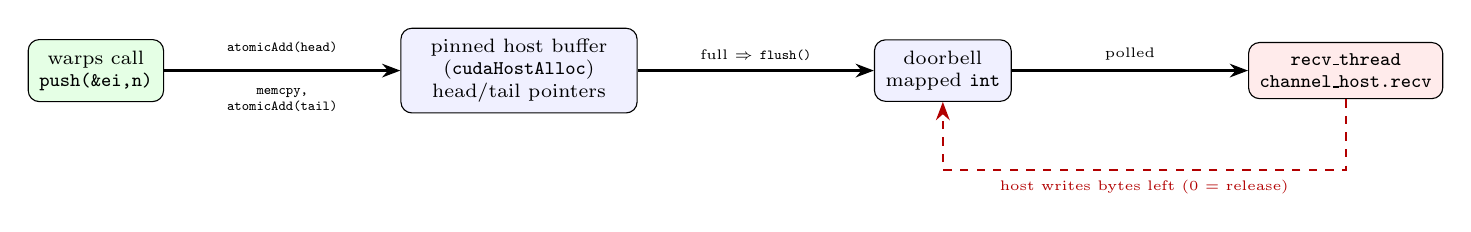
\begin{tikzpicture}[node distance=8mm and 30mm]
\node[gbox] (w) {warps call\\\texttt{push(\&ei,n)}};
\node[box,right=of w,minimum width=3cm] (buf) {pinned host buffer\\(\texttt{cudaHostAlloc})\\head/tail pointers};
\node[box,right=of buf] (db) {doorbell\\mapped \texttt{int}};
\node[rbox,right=of db] (r) {\texttt{recv\_thread}\\\texttt{channel\_host.recv}};
\draw[arr](w)--(buf);
\node[lbl,above=1mm of $(w.east)!0.5!(buf.west)$] {\texttt{atomicAdd(head)}};
\node[lbl,below=1mm of $(w.east)!0.5!(buf.west)$] {\texttt{memcpy,}\\\texttt{atomicAdd(tail)}};
\draw[arr](buf)--node[lbl,above]{full $\Rightarrow$ \texttt{flush()}}(db);
\draw[arr](db)--node[lbl,above]{polled}(r);
\draw[arr,dashed,red!70!black] (r.south) -- ++(0,-0.9) -| node[lbl,below,pos=0.25]{host writes bytes left (0 = release)} (db.south);
\end{tikzpicture}}

\small\raggedright
\textbf{push:} reserve space with \texttt{atomicAdd} on the head; if it runs past \texttt{buff\_end}, the first warp to notice waits for tail==its pointer and calls \texttt{flush()}; others spin until head is reset.\\
\textbf{flush:} \texttt{\_\_threadfence\_system()}; \texttt{*doorbell = nbytes}; \textbf{spin until host sets doorbell to 0}; reset tail then head.
\end{frame}

\begin{frame}{Receiver: \texttt{recv} and the thread loop}
\small
\texttt{ChannelHost::recv(buf, max)}: read \texttt{*doorbell}; 0 $\Rightarrow$ return 0. Else copy $\min(n,\texttt{max})$ bytes from the pinned buffer (read head advances); write \texttt{*doorbell = bytes\_left}. When it reaches 0 the GPU resumes. Since \texttt{max = sizeof(exception\_info)}, the host drains \emph{one packet at a time}, each time re-arming the doorbell with the bytes left.

\medskip
\texttt{recv\_thread\_fun} (\texttt{nixnan.cu}):
\begin{itemize}
\item busy loop while \texttt{recv\_thread\_started}; works only if \texttt{recv\_thread\_receiving} (set at kernel launch).
\item \texttt{to\_skip()} packets are stepped over (\texttt{continue}).
\item \texttt{warp()==-1} $\Rightarrow$ \texttt{recv\_thread\_receiving=false} (the sentinel).
\item otherwise decode and \texttt{nnout\_line()} (mutex-guarded, flushed; avoids torn lines).
\item \texttt{MAX\_ERRORS} reached $\Rightarrow$ \texttt{nnterminate}.
\end{itemize}
\end{frame}

\begin{frame}{Receiver state machine}
\centering
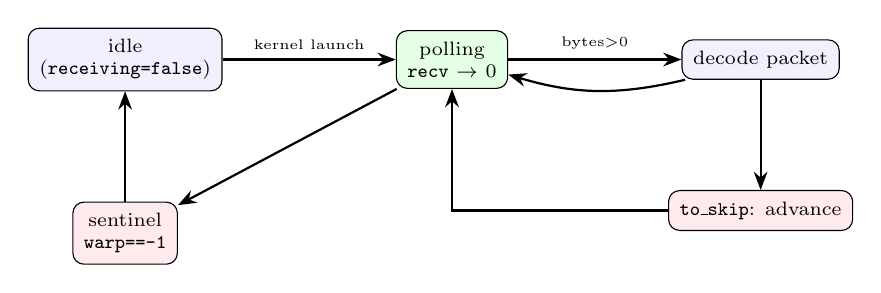
\begin{tikzpicture}[node distance=14mm and 22mm,every node/.style={font=\scriptsize}]
\node[box] (idle) {idle\\(\texttt{receiving=false})};
\node[gbox,right=of idle] (poll) {polling\\\texttt{recv} $\to$ 0};
\node[box,right=of poll] (dec) {decode packet};
\node[rbox,below=of dec] (skip) {\texttt{to\_skip}: advance};
\node[rbox,below=of idle] (sent) {sentinel\\\texttt{warp==-1}};
\draw[arr](idle)--node[above,lbl]{kernel launch}(poll);
\draw[arr](poll)--node[above,lbl]{bytes>0}(dec);
\draw[arr](dec)--(skip);
\draw[arr](skip)-|(poll);
\draw[arr](dec) to[bend left=15] (poll);
\draw[arr](poll)--(sent);
\draw[arr](sent)--(idle);
\end{tikzpicture}

\small Why \texttt{skip}? The channel buffer is exactly one packet (\texttt{CHANNEL\_SIZE}), and \texttt{push} only flushes when the \emph{next} packet does not fit. So a lone real packet would sit unflushed. Each first occurrence is therefore pushed twice: the real one (\texttt{skip=0}) and a dummy (\texttt{skip=1}) whose arrival forces the real one out; the receiver steps over the dummy. (My reading of the code; no comment in the repository states the intent. It is consistent with all observed runs, see the sentinel slide.)
\end{frame}

\begin{frame}[fragile]{The ``one last message'': sentinel flush --- design vs.\ this commit}
\begin{lstlisting}
__global__ void flush_channel() {
  exception_info ei(int4{-1,-1,-1,-1}, 0,0,0,0);   // warp() == -1
  channel_dev.push(&ei, sizeof(exception_info));
  channel_dev.flush();
}
\end{lstlisting}
\small
\begin{itemize}
\item \textbf{Design:} after each kernel, launch \texttt{flush\_channel<<<1,1>>>}, so (a) any partially filled buffer is flushed and (b) the receiver sees \texttt{warp==-1} and clears \texttt{recv\_thread\_receiving}; the exit callback then waits \texttt{while(recv\_thread\_receiving) sched\_yield();} so no report is lost and the doorbell spin cannot hang on a half-drained buffer.
\item \textbf{Status in commit \texttt{ce35185}:} the launch of \texttt{flush\_channel}, the \texttt{skip\_flag} toggling and the wait loop in \texttt{nvbit\_at\_cuda\_event} are \textbf{commented out}. The receiver still understands the sentinel, but nothing sends it. The exit callback now only does \texttt{cudaDeviceSynchronize()} and an error check.
\item \textbf{Checked:} in the three \texttt{rd\_tc} runs the live \texttt{error [\ldots]} lines match the final report per flag (e.g.\ fp16acc32: NaN 50 live $=16$ f16 $+\,34$ f32; Inf 12 $=8+4$; bf16acc32: NaN $66=24+42$, Inf $36=16+20$). No first occurrence was lost in these runs. This does not prove the sentinel is unnecessary: the dummy \texttt{skip} packet may be what makes it work, and the last dummy always stays in the buffer.
\end{itemize}
\end{frame}

\begin{frame}{End of run}
\small
\begin{itemize}
\item \texttt{nvbit\_at\_ctx\_term}: \texttt{recv\_thread\_started=false}; \texttt{join}.
\item \texttt{recorder->end()}: \texttt{cudaMemcpy} \texttt{device\_errors} $\to$ \texttt{host\_errors}.
\item For every (inst, operand, flag-set) with count $>$ 0: bucket by (type, is\_mem) and by flag (NaN, Inf, -Inf, Sub, Div0): \emph{distinct locations} = number of buckets hit, \emph{repeats} = total $-$ distinct.
\item Printed as ``\texttt{------------ nixnan Report -----------}'' with FP16/BF16/FP32/FP64 sections (and memory sections).
\end{itemize}
Note the live lines show each (instruction, operand, flag-set) \emph{once}; the table gives how many times it recurred.
\end{frame}

\section{Part A}
\begin{frame}[fragile]{Part A --- an ordinary SASS instruction: \texttt{HFMA2} (\texttt{rd\_step\_fp16})}
\small Real SASS from \texttt{cuobjdump -sass rd\_nixnan}:
\begin{lstlisting}
/*0130*/ HFMA2 R0, R0.H0_H0, c[0x0][0x170].H0_H0, R9.H0_H0 ;
\end{lstlisting}
\nn{} (\texttt{TOOL\_VERBOSE=1}) logged:
\begin{lstlisting}
Instrumenting instruction HFMA2 R0, R0.H0_H0, c[0x0] [0x170].H0_H0, R9.H0_H0 ;
Instrumenting instruction with 2 registers          <- AFTER: reginfo + 1 reg
Instrumenting operand 0. div0: 0, regs: 1, count: 2
Instrumenting instruction with 6 registers          <- BEFORE: 3 reginfo + 3 regs
Instrumenting operand 1. div0: 0, regs: 1
Instrumenting operand 2. div0: 0, regs: 1
Instrumenting operand 3. div0: 0, regs: 1
\end{lstlisting}
\begin{itemize}\small
\item Four groups: D=\texttt{R0} (1 reg, 2 halves), A=\texttt{R0}, B=\textbf{constant bank} \texttt{c[0x0][0x170]}, C=\texttt{R9}. Operand~2 is read with \texttt{nvbit\_add\_call\_arg\_cbank\_val}.
\item AFTER: \texttt{arg\_count} = 1 reginfo + 1 reg = 2. BEFORE: 3 reginfo + 3 regs = 6.
\end{itemize}
\end{frame}

\begin{frame}[fragile]{Part A --- what came back}
\small Report lines for this instruction (first occurrences, real output):
\begin{lstlisting}
error [infinity] detected in operand 1 of instruction HFMA2 R0, R0.H0_H0, c[0x0] [0x170].H0_H0, R9.H0_H0 ; in function rd_step_fp16 of type f16
error [infinity] detected in operand 0 of instruction HFMA2 R0, R0.H0_H0, c[0x0] [0x170].H0_H0, R9.H0_H0 ; in function rd_step_fp16 of type f16
\end{lstlisting}
\begin{itemize}\small
\item Operand~1 inf (a \emph{source}, checked BEFORE): the previous step's overflow arrived in the input.
\item Operand~0 inf (the \emph{destination}, checked AFTER): the multiply-add itself produced/propagated it.
\item No \texttt{at file:line}: \texttt{rd\_nixnan} was built without \texttt{-lineinfo}, so \texttt{nvbit\_get\_line\_info} returns nothing and the location is omitted.
\item The type shown, \texttt{f16}, comes from the stored \texttt{opertypes[op]}, not from the packet (\texttt{tp\_override=UNKNOWN}).
\end{itemize}
Also visible in the same log: \texttt{STG.E.U16} gets ``Unsupported store instruction'' (memory instrumentation is off unless \texttt{INSTR\_MEM=1}).
\end{frame}

\section{Part B}
\begin{frame}[fragile]{Part B --- \texttt{HMMA.16816.F16}: one warp instruction, four register groups}
\begin{lstlisting}
/*0840*/ HMMA.16816.F16 R26, R4, R30, R26 ;      // cuobjdump -sass rd_tc
\end{lstlisting}
\begin{lstlisting}
Instrumenting instruction with 3 registers      <- AFTER:  1 reginfo + 2 regs
Instrumenting operand 0. div0: 0, regs: 2, count: 4
Instrumenting instruction with 11 registers     <- BEFORE: 3 reginfo + 8 regs
Instrumenting operand 1. div0: 0, regs: 4
Instrumenting operand 2. div0: 0, regs: 2
Instrumenting operand 3. div0: 0, regs: 2
\end{lstlisting}
\small (Verbatim lines from the log for other HMMAs of the same kernel; they are identical for every \texttt{HMMA.16816.F16}.)
\end{frame}

\begin{frame}{Part B --- which registers are picked up}
\centering
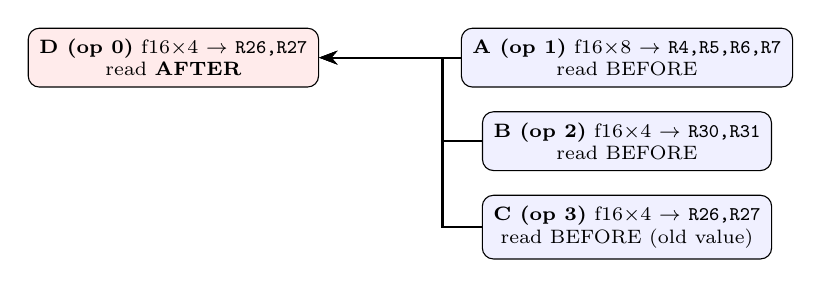
\begin{tikzpicture}[node distance=3mm,every node/.style={font=\scriptsize}]
\node[rbox,minimum width=3.4cm] (d) {\textbf{D (op 0)} f16$\times$4 $\to$ \texttt{R26,R27}\\read \textbf{AFTER}};
\node[box,minimum width=3.4cm,right=18mm of d] (a) {\textbf{A (op 1)} f16$\times$8 $\to$ \texttt{R4,R5,R6,R7}\\read BEFORE};
\node[box,minimum width=3.4cm,below=of a] (b) {\textbf{B (op 2)} f16$\times$4 $\to$ \texttt{R30,R31}\\read BEFORE};
\node[box,minimum width=3.4cm,below=of b] (c) {\textbf{C (op 3)} f16$\times$4 $\to$ \texttt{R26,R27}\\read BEFORE (old value)};
\draw[arr](a.west)--++(-0.5,0)|-(d.east);\draw[arr](b.west)--++(-0.5,0)|-(d.east);\draw[arr](c.west)--++(-0.5,0)|-(d.east);
\end{tikzpicture}

\small\raggedright
$m16n8k16$ half-precision: per thread the A fragment is 8 halves (4 registers), B 4 halves (2), C/D 4 halves (2). Starting registers come from the SASS text (\texttt{R4}, \texttt{R30}, \texttt{R26}); \nn{} takes \texttt{reg\_start + i} for $i<\texttt{num\_regs}$. Consequently the 8 BEFORE registers plus 3 reginfo words = 11 call arguments; the AFTER call has 3.
Every active lane of the warp supplies its own copy (the device function runs per thread, then ORs across lanes).
\end{frame}

\begin{frame}[fragile]{Part B --- reginfo words for this HMMA (verified offline)}
\small Using the layout above (count, type, h0, h1, operand, num\_regs):
\begin{center}\begin{tabular}{@{}cccl@{}}
operand & count & num\_regs & word\\\hline
0 (D) & 4 & 2 & \texttt{0x00010C04}\\
1 (A) & 8 & 4 & \texttt{0x00022C08}\\
2 (B) & 4 & 2 & \texttt{0x00014C04}\\
3 (C) & 4 & 2 & \texttt{0x00016C04}\\
\end{tabular}\end{center}
\textbf{Verification:} the words were produced by compiling the real \texttt{reginfo.cuh} with g++ and filling the fields as \texttt{get\_reginfo} does (all fields zeroed first). They match my hand computation. They were \emph{not} dumped from the running tool; the tool leaves the 12 reserved bits uninitialised, which the device code ignores. For \texttt{.F32}: D $=$ \texttt{0x00020C84}, C $=$ \texttt{0x00026C84}.

\bigskip
Limits worth knowing: \texttt{num\_regs} has 4 signed bits; \texttt{get\_reginfo} asserts \texttt{get\_num\_regs<16}. HMMA.1684 TF32 and \texttt{.F32}/\texttt{.F32.BF16} variants have their own entries (f32 count 4 for D and C).
\end{frame}

\begin{frame}[fragile]{Part B --- what \nn{} reported (real output, \texttt{fp16acc16})}
\begin{lstlisting}
error [infinity] detected in operand 0 of instruction HMMA.16816.F16 R26, R4, R30, R26 ; ...
error [infinity] detected in operand 0 of instruction HMMA.16816.F16 R4, R8.reuse, R4, R22 ; ...
error [infinity] detected in operand 3 of instruction HMMA.16816.F16 R6, R8, R6, R26 ; ...
  step 230: max|finite|=6.5280e+04  inf=120  nan=0          (program's own count)
error [NaN] detected in operand 0 of instruction HMMA.16816.F16 R22, R16, R22, R8 ; ...
\end{lstlisting}
\small
\begin{itemize}
\item Operand 0 inf: the tensor core \emph{produced} the overflow in its f16 accumulator (step 230).
\item Next step: inf inputs meet the zeros of $P$: $0\times\infty$ = NaN inside HMMA; all 4096 entries are NaN one step later.
\item With \texttt{fp16acc32}/\texttt{bf16acc32} the first inf is born in \texttt{F2FP.PACK}/\texttt{F2FP.BF16.PACK}. \textbf{Verified:} \texttt{grep -c F2FP instructions.json} $=0$ and the logs contain no \texttt{F2FP} line, so that conversion is not instrumented; \nn{} first shows the inf as an operand of the \emph{next} HMMA.
\item \texttt{LINE\_INFO=1} did not give \texttt{mma\_sync} source lines in these runs (no \texttt{at file:line}).
\end{itemize}
\end{frame}

\begin{frame}{Summary}
\small
\begin{itemize}
\item Tool is a table: opcode $\to$ operand groups (type, count); everything else is generic.
\item One 32-bit \texttt{reginfo} per operand; the GPU function is variadic.
\item Two injected calls: destination AFTER, sources BEFORE.
\item Warp-level OR, per-site atomic counters; only \emph{first} occurrences cross the channel.
\item Channel = pinned buffer + doorbell handshake; one polling receiver thread; sentinel in design but disabled in this commit.
\item HMMA fits unchanged: it is just an opcode with four groups and 11 BEFORE arguments.
\end{itemize}
Files: \texttt{rd\_nixnan/latex/data/} (raw logs), \texttt{nixnan-walkthru-report.pdf} (prose).
\end{frame}
\end{document}
